\documentclass{article}

\usepackage{microtype}
\usepackage{graphicx}
\usepackage{booktabs}
\usepackage{hyperref}
\newcommand{\theHalgorithm}{\arabic{algorithm}}
\usepackage{icml2026}
\usepackage{algorithm}
\usepackage{algorithmic}

\usepackage{amsmath,amssymb,mathtools,amsthm}
\usepackage[shortlabels]{enumitem}
\usepackage{xcolor}
\usepackage{float}
\usepackage[capitalize,noabbrev]{cleveref}

\theoremstyle{plain}
\newtheorem{theorem}{Theorem}[section]
\newtheorem{proposition}[theorem]{Proposition}
\newtheorem{lemma}[theorem]{Lemma}
\newtheorem{corollary}[theorem]{Corollary}
\theoremstyle{remark}
\newtheorem{remark}[theorem]{Remark}
\newcommand{\E}{\mathbb E}
\graphicspath{{../../docs/figures/}}
\newcommand{\pending}[1]{\textcolor{red}{[#1]}}

\icmltitlerunning{Faster, Not More Diverse}
\makeatletter\newcommand{\setrunninghead}{\gdef\@icmltitlerunning{Faster, Not More Diverse}}\makeatother

\begin{document}

\twocolumn[
  \icmltitle{Faster, Not More Diverse: What Moves the Accuracy--Diversity\\ Frontier in RL with Verifiable Rewards}
  \setrunninghead
  \begin{icmlauthorlist}
    \icmlauthor{Anonymous Authors}{anon}
  \end{icmlauthorlist}
  \icmlaffiliation{anon}{Anonymous Institution}
  \icmlcorrespondingauthor{Anonymous Authors}{anon@anon}
  \icmlkeywords{reinforcement learning with verifiable rewards, policy gradient variance, pass@k, evaluation, exploration}
  \vskip 0.3in
]
\printAffiliationsAndNotice{}

\begin{abstract}
Many variants of reinforcement learning with verifiable rewards (RLVR) change how sampled answers are scored and report higher pass@$k$. They are almost always compared at the same training step, where a method that learns more slowly is also less sharpened, and therefore looks more diverse. We compare methods at matched pass@1 instead, in pre-registered experiments with bootstrap intervals over problems. For any advantage rule that depends only on correctness, we show that the expected update on each problem is a scalar multiple of the gradient of its success probability, and we derive the second moment in terms of four measurable quantities; incorrect answers carry 2--3 times larger squared score norms than correct ones. Across two model families, negative-sample reinforcement, positive-sample reinforcement, constant baselines, a pass@$k$ objective and the published unlikeliness reward all lie within about two points of pass@16 of one trajectory, and injecting zero-mean noise of the predicted size into positive reinforcement reproduces the slower progress of negative reinforcement. The same holds for interventions that add samples rather than reweight them: replaying successes moves the frontier by about one point, and quadrupling the rollouts per problem reaches the point that Dr.\ GRPO reaches with more steps. A per-problem log-odds model initialized from base-model success counts reproduces the frontier of nine further rules and of a second model family within two points. \pending{Final sentence: what moves the frontier (Pre-registrations 18 and 19).}
\end{abstract}

\section{Introduction}
RL with verifiable rewards trains a language model on problems whose answers can be checked automatically. The update is a sum over sampled answers, $g=\sum_i A_i\nabla\log\pi(y_i)$, in which the advantage $A_i$ depends on whether answer $i$ was correct. A large literature varies the advantages: rewarding only correct answers or penalizing only incorrect ones \citep{zhu2025nsr}, removing normalizations \citep{liu2025drgrpo}, filtering or reallocating rollouts \citep{yu2025dapo,xiong2025reinforceada}, adding exploration bonuses \citep{he2025unlikely}, or aiming at pass@$k$ directly \citep{walder2025pkpo,thrampoulidis2025shaping}. Most of these changes are motivated by diversity, measured as pass@$k$ at large $k$, which RL training is known to reduce relative to the base model \citep{yue2025limit}.

These methods are usually evaluated at a fixed number of training steps. That comparison has a blind spot. A variant that progresses more slowly is, at any given step, less sharpened than its competitor, and its pass@$k$ is higher for that reason alone. What matters is the trade-off itself: how much pass@$k$ a method retains at a given level of accuracy. We therefore compare methods at matched pass@1, interpolating along a reference run's trajectory and its temperature envelope, with intervals from a problem-level bootstrap and decision rules fixed before each experiment.

Seen this way, most of the field's diversity gains disappear. Our first result is theoretical. For every rule whose advantages and sampling decisions depend only on correctness, the expected update on a problem $x$ is $c(p_x)\nabla p_x$, where $p_x$ is the problem's success probability; rules differ in the per-problem coefficient $c$ and in the second moment of the update, for which we give an exact expression. Positive-only and negative-only reinforcement have the same mean and differ by a zero-mean term, which is large because incorrect answers have larger score norms. Our second result is empirical. Across Qwen2.5-Math-1.5B and OLMo-2-1B, the advantage rules we tested lie on one trajectory in the (pass@1, pass@16) plane, and adding zero-mean noise of the predicted size to positive reinforcement reproduces the slower progress of negative reinforcement. Noise sets how fast a run moves along the trajectory; it does not move the trajectory.

The diversity measure itself explains why. At matched pass@1, pass@$k$ is a concave average of per-problem success, so it measures only how evenly success is spread across problems. Raising it requires signal on problems the policy rarely solves, and a group of eight rollouts on such a problem usually contains no correct answer, so there is nothing to reweight. We therefore test interventions that add signal rather than reweight it: replay of stored successes, replay seeded with base-model successes, a supervised warm start on those successes, and four times as many rollouts per problem. These move the frontier by about one point at most, and groups of 32 rollouts reach exactly the point that Dr.\ GRPO reaches when trained longer. In this regime, the interventions people use make training faster, not more diverse. A two-parameter model of per-problem log-odds learning, initialized from base-model success counts, reproduces the frontier of nine further rules and of the second model family within two points, though it underestimates how far the frontier keeps rising beyond the range it was fitted on. \pending{Pre-registrations 18--19: rollout allocation by frontier value and external information.}

All experiments were pre-registered, and each design was reviewed independently before launch; registrations, analysis code and failed predictions are reported (\cref{app:prereg}).

\section{Setup and the matched-accuracy protocol}\label{sec:setup}
For a problem $x$ with reward $r\in\{0,1\}$, the policy's success probability is $p_x=\Pr_\pi(r=1\mid x)$, the score of an answer is $\ell(y)=\nabla_\vartheta\log\pi(y\mid x)$, and $F_r=\E[\|\ell\|^2\mid r]$ is the mean squared score norm of correct ($r=1$) and incorrect ($r=0$) answers. Each training step samples $G=8$ rollouts for each of 16 problems. Dr.\ GRPO uses $A_i=r_i-\bar r$ within a group \citep{liu2025drgrpo}; positive-sample reinforcement (PSR) uses $A_i=r_i$ and negative-sample reinforcement (NSR) $A_i=r_i-1$ \citep{zhu2025nsr}. Over $N$ problems,
\begin{align*}P_k&=\tfrac1N\textstyle\sum_x\big[1-(1-p_x)^k\big],\\ \widehat P_k&=\tfrac1N\textstyle\sum_x\Big[1-\binom{n_x-C_x}{k}\Big/\binom{n_x}{k}\Big],\end{align*}
where $\widehat P_k$ is the unbiased estimator from $C_x$ correct answers among $n_x=32$ samples \citep{chen2021codex}.

\begin{proposition}[pass@$k$ at matched pass@1 measures spread]\label{prop:spread}
$P_1=\E_x p_x$ and $P_k=\E_x f_k(p_x)$ with $f_k(p)=1-(1-p)^k$ strictly concave for $k>1$. Among distributions of $\{p_x\}$ with the same mean, a mean-preserving spread lowers $P_k$; $P_k$ is largest when all $p_x$ are equal.
\end{proposition}

\textbf{Protocol.} For a checkpoint with pass@1 $a$, the reference value is $E_B(a)=\max\{L_{\rm steps}(a),L_T(a)\}$: the larger of the linear interpolations in pass@1 along Dr.\ GRPO's trajectory (base model and steps 50, 100, 150) and along its step-150 temperature sweep ($T\in\{1,1.15,1.3\}$), each within its supported range. A run's gain is the mean of $\widehat P_{16}-E_B(a)$ over its checkpoints inside the reference range, averaged over seeds; intervals come from 2,000 bootstrap draws over problems with the reference recomputed in every draw. We call a difference \emph{average equivalence} if its 90\% interval lies within $\pm2$ points and say a method \emph{moves the frontier} if its gain is at least $+2$ points with the 95\% interval above zero in every seed. Runs that share a seed see the same problems at every step.

\section{Theory}\label{sec:theory}
\begin{theorem}[Two moments of correctness-only rules]\label{thm:moments}
Let a rule draw answers i.i.d.\ from $\pi(\cdot\mid x)$, stop at a time $N\le n_{\max}$ that depends only on the rewards observed so far, and assign advantages that depend only on the rewards. Then $g=\sum_{i\le N}A_i\ell(y_i)$ satisfies
\begin{align*}\E g&=c(p)\nabla p,\\ \E\|g\|^2&=F_1D_1(p)+F_0D_0(p)+\|\nabla p\|^2X(p),\end{align*}
where $c$, $D_1$, $D_0$, $X$ and $\E N$ depend only on the rule and on $p$.
\end{theorem}
The proof conditions on the reward sequence, given which $N$ and the advantages are fixed and $\E[\ell\mid r=1]=\nabla p/p$, $\E[\ell\mid r=0]=-\nabla p/(1-p)$ (\cref{app:proofs}). For fixed groups the mean part is known \citep{davis2025objective}, and the equality of the PSR and NSR means is classical baseline invariance \citep{williams1992,greensmith2004}. The second-moment part, with $F_0\neq F_1$ and reward-dependent stopping, is what lets us predict and manipulate noise.

\begin{corollary}\label{cor:psrnsr}
With advantage $a$ for correct and $b$ for incorrect answers in a group of $n$, $\E g=n(a-b)\nabla p$. PSR and NSR have the same mean $n\nabla p$, and NSR equals PSR plus the zero-mean term $-\sum_i\ell(y_i)$; when $F_0>F_1$, NSR has the larger second moment on every problem with $p<F_0/(F_0+F_1)$.
\end{corollary}

\begin{lemma}[Rarely solved problems receive sparse updates]\label{lem:starve}
Under Dr.\ GRPO with a group of $n$, the update on problem $x$ is zero unless the group contains both a correct and an incorrect answer, which happens with probability $1-p^n-(1-p)^n\approx np$ for small $p$. Any reweighting of the advantages by a function of the group's rewards leaves this probability unchanged.
\end{lemma}

Two consequences frame the experiments. A correctness-only rule can only reweight problems and change the noise of the update. Since the expected update on every problem points along $\nabla p_x$, one might expect all such rules to trace one trajectory, but cross-problem reweighting can rotate the aggregate update through shared parameters \citep{barakat2026interference}, so whether they do is an empirical question. And by \cref{prop:spread} and \cref{lem:starve}, moving the frontier requires realized signal on problems with small $p_x$, which reweighting cannot create.

\section{Advantage rules share one trajectory}\label{sec:audit}
\textbf{Models.} Qwen2.5-Math-1.5B \citep{yang2024qwen25math}: 3,920 MATH training problems, 150 steps, answers up to 512 tokens, evaluation on 511 held-out MATH test problems. OLMo-2-0425-1B-SFT \citep{olmo2024}: 300 steps, 256 held-out problems, 1,024 tokens. AdamW at $10^{-6}$, strictly on-policy updates with sequence-sum losses. All answer keys were audited (\cref{app:labels}).

\textbf{Incorrect answers carry larger gradients.} Measured on full-parameter scores before training, $F_0/F_1$ is 2.14 and 2.54 on OLMo and 2.7--3.4 on Qwen; it falls to about 1.4--1.6 during training. With $F$ re-measured during training, \cref{thm:moments} predicts the measured second moment of the update within a factor of 0.69--1.18. NSR's measured noise is about 6 times PSR's on Qwen and 19--22 times on OLMo.

\textbf{NSR is a slower PSR.} NSR progresses more slowly than PSR and ends with the same pass@64. At matched pass@1 the two are equivalent on average on both families (\cref{tab:audit}); the original implementation of \citet{zhu2025nsr}, with sample reuse, clipping and token averaging, does not reproduce the reported advantage either. Constant baselines $A=r-b$ with the same mean order their progress rates by the noise the theorem predicts (rank correlation 0.9--0.97) and stay within about two points of PSR's trajectory.

\begin{table}[t]
\caption{Matched-pass@1 differences in pass@16 (points; 90\% bootstrap intervals over problems, pooled over seeds).}
\label{tab:audit}
\centering\small
\resizebox{\columnwidth}{!}{\begin{tabular}{@{}llr@{}}
\toprule
Comparison & Model, seeds & Difference [90\%]\\
\midrule
NSR vs PSR & OLMo, 2 & $-0.30$ [$-1.28$, $+0.77$]\\
NSR vs PSR & Qwen, 3 & $-0.20$ [$-0.97$, $+0.55$]\\
PSR + matched noise vs PSR & Qwen, 3 & $-0.37$ [$-1.13$, $+0.46$]\\
NSR at $2\times$ learning rate vs PSR & Qwen, 3 & $-0.03$ [$-0.88$, $+0.88$]\\
pass@4 objective vs Dr.\ GRPO & OLMo, 2 & $+1.32$ [$+0.24$, $+2.26$]\\
\bottomrule
\end{tabular}}
\end{table}

\textbf{Noise is sufficient for the lag.} Same-mean baselines change the noise and the systematic push on incorrect answers together. To separate them we add to PSR a random-sign term whose magnitude, at every step, matches NSR's predicted second moment; it has mean zero and pushes no answer systematically. On a pre-registered progress index on which NSR is 0 and PSR is 1, PSR with this noise is at $\phi=-0.11$, 90\% $[-0.22,-0.05]$: noise of NSR's size reproduces NSR's lag. NSR at twice the learning rate reaches PSR's rate ($\phi=1.16$). Under Adam the added noise does not shrink the steps; it reduces their alignment with the expected update by 13--27\%.

\textbf{The trajectory is not a temperature effect.} If RL simply sharpened next-token distributions, a late checkpoint sampled at a higher temperature should lie above the training trajectory. It does not: the difference at matched pass@1 is $-1.42$, 90\% $[-2.19,-0.68]$, and entropy on fixed base-model text barely changes during training (1.081 to 1.064) while entropy on the policy's own samples falls three- to fourfold. Training moves the policy onto high-confidence paths rather than sharpening it uniformly.

\textbf{Other correctness-only interventions.} A pass@4 objective \citep{walder2025pkpo} stays on the trajectory on Qwen ($+1.6$ and $+0.2$ in two seeds) and is slightly above it on OLMo. The unlikeliness reward \citep{he2025unlikely} gives $+0.14$ points, 95\% $[-0.32,+0.62]$ (three seeds). Entropy bonuses gave no gain in a pilot, and entropy floors and adaptive entropy control stopped training from progressing.

\section{Adding signal makes training faster}\label{sec:faster}
\Cref{lem:starve} says the missing ingredient is realized signal on rarely solved problems. We test four ways of supplying it, on three fresh seeds, against Dr.\ GRPO at matched pass@1.

\textbf{Replay.} Storing verified successes and replaying them with a log-likelihood term, choosing problems in proportion to the posterior mean of $k\,p(1-p)^{k-1}=\partial f_k/\partial\log p$, gives $+1.19$ points, 95\% $[+0.54,+1.79]$; uniform replay gives $+0.61$. Seeding the replay archive with successes from 32 base-model samples per problem gives $+1.02$, 95\% $[+0.23,+1.68]$, while lowering step-150 pass@1 by 5.35 points. All three are average agreement under the registered rule.

\textbf{More rollouts, and a warm start.} Dr.\ GRPO with groups of 32 and a supervised warm start on the base-model successes both end at pass@1 52.5 after 150 steps, outside the range Dr.\ GRPO reaches in that time (44.1), so the registered comparison is undefined. A 450-step Dr.\ GRPO run provides the missing reference (\cref{fig:frontier}). Against it, groups of 32 lie on the trajectory ($+0.60$ points, against $+0.47$ for the 150-step Dr.\ GRPO runs, which reflects the reference seed's own noise); four times as many rollouts buy speed, not a better trade-off. The warm start lies about two points above the long trajectory ($+2.38$); this is the largest departure we have observed, and it is the only intervention that trains on correct solutions to many problems at once. \pending{Long-run reference with three seeds; interval.}

\begin{figure}[t]
\centering
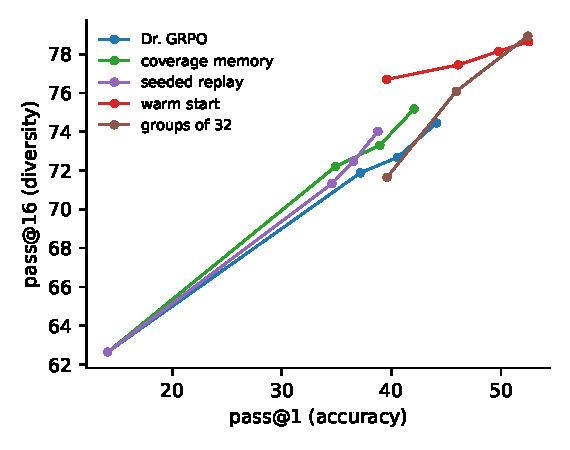
\includegraphics[width=\columnwidth]{frontier_qwen.pdf}
\caption{Seed-mean (pass@1, pass@16) trajectories on Qwen. Replay variants stay close to Dr.\ GRPO; groups of 32 and the warm start end near (52.5, 79), which Dr.\ GRPO reaches with longer training. \pending{Add the 450-step trajectory.}}
\label{fig:frontier}
\end{figure}

\section{A per-problem model of the frontier}\label{sec:model}
If every rule moves problems along their own gradients at a rate set by sampled successes, the frontier should be predictable from the base model's success counts alone. We model each problem's log-odds as starting at an empirical-Bayes estimate from 32 base-model samples and evolving as
\[\dot\theta_x=p_x(1-p_x)+\tau\,\tfrac1N\textstyle\sum_{x'}p_{x'}(1-p_{x'}),\]
own-problem growth plus a uniform transfer term. A checkpoint is placed where the model's mean success equals its observed pass@1, and the model predicts everything else. We fitted $\tau=-0.20$ once on Dr.\ GRPO's nine checkpoints, froze it, and evaluated it on pre-registered test sets.

The frozen model predicts pass@16 for nine further rules on Qwen with a root-mean-square error of 1.21 points (56 checkpoints), for five rules on OLMo with $\tau$ carried over from Qwen at 1.90 points (50 checkpoints), and at a 1,024-token budget at 0.85 points (\cref{fig:law}). Simpler alternatives fit far worse: a uniform log-odds shift misses by 9--21 points and an affine log-odds map, fitted on the same data, by up to 12.6. The model also explains why the frontier collapses: under a uniform shift, problems the base model never solved in 32 samples would reach 70--80 pass@16, while the model and the data put them at 24. Success concentrates on problems that were already partly solved.

The model has clear limits. It fails its registered criterion after the supervised warm start (3.56 points), where problems the base never solved gain about 12 points less than predicted. It also underestimates how far the frontier keeps rising: on the 450-step run it is 2.0 and 3.6 points too low at steps 200 and 250. With 256 further base samples on the hardest problems the fitted transfer coefficient becomes $+0.20$, 90\% $[+0.10,+0.35]$, so learning on one problem does carry over to others, weakly. We use the model as a description of the frontier within the trained range, not as a law that extrapolates.

\begin{figure}[t]
\centering
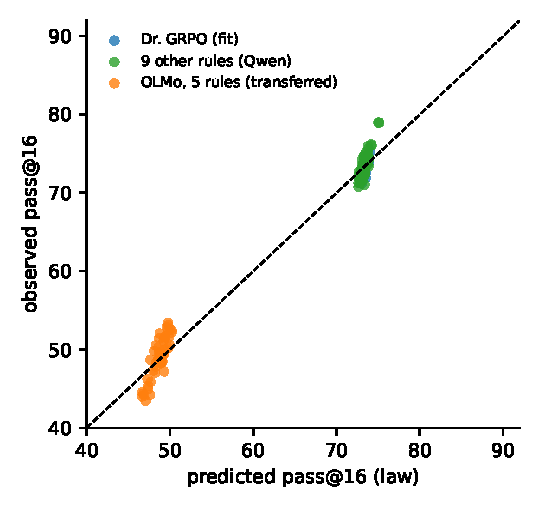
\includegraphics[width=0.8\columnwidth]{law_fit.pdf}
\caption{Predicted against observed pass@16 for the frozen per-problem model.}
\label{fig:law}
\end{figure}

\section{What moves the frontier}\label{sec:moves}
\pending{Pre-registration 18: rollout allocation at an equal rollout budget, by frontier value (AC), by per-rollout signal (AV) and by HORA's hit utility (HR); forecasts registered in advance (AC $+2.6$ to $+4.3$, HR about 0, AV $-0.7$ to $-1.1$). Pre-registration 19: human-written solutions on problems the base never solved versus on problems it did, at equal size.}

\section{Related work}

\paragraph{Advantage design and sample polarity.}
\citet{zhu2025nsr} report better high-$k$ pass@$k$ retention under negative sample reinforcement (NSR) than positive sample reinforcement (PSR). Subsequent work examines negative-sample exploration \citep{tang2025polarity} and asymmetric or difficulty-dependent advantages \citep{ingle2026negative,yu2026symmetry,decugis2026fade}. The original NSR--PSR comparison motivates our matched-pass@1 test on two model families. On Qwen, trace-matched zero-mean sign noise added to PSR reproduces NSR's pooled early accuracy lag, with seed heterogeneity. This establishes a perturbation that can reproduce the lag without separately identifying scalar noise magnitude and covariance structure.

\paragraph{The objective view of RLVR.}
Binary-reward updates can be expressed as ascent on monotone transforms of per-problem success \citep{davis2025objective}. This objective view also appears in surrogate-reward interpretations of advantage shaping \citep{thrampoulidis2025shaping} and analyses of weights that minimize time to target accuracy \citep{heckel2026weighting}. Pass@$k$ policy gradients are reweighted pass@1 gradients \citep{yu2025diagnostic}. Our extension is an exact per-problem second moment for correctness-only rules under independent sampling, allowing reward-dependent stopping and unequal conditional mean squared score-function norms $F_0$ and $F_1$. Shared parameters allow changes in prompt weights to rotate aggregate updates \citep{barakat2026interference}, so the mean identity does not imply a common frontier.

\paragraph{Diversity, pass@$k$, and evaluation.}
DARS already plots pass@1--pass@$K$ trajectories and reports higher pass@128 at fixed pass@1, without intervals or a registered matching protocol \citep{yang2025depth}. We add pre-registered decision criteria and problem-level bootstrap intervals that recompute the interpolated reference within shared pass@1 support. Base--RLVR pass@$k$ crossovers \citep{yue2025limit} and confidence bands for them \citep{yang2026kernel} make evaluation uncertainty relevant to these comparisons. CoT-pass@$k$ instead evaluates intermediate reasoning \citep{wen2025cotpassk}; BBG gates updates by posterior marginal pass@$k$ utility \citep{yuan2026overtraining}. At matched pass@1, pass@$k$ summarizes the cross-problem distribution of success probabilities. Our model predicts aggregate pass@16 using base success counts, observed checkpoint pass@1, and a transfer coefficient frozen before computing test predictions across rules, model families, and evaluation budgets. Its registered warm-start failure limits this description, while ``RLVR is a Kernel'' challenges deterministic prediction from base success more generally \citep{yang2026kernel}.

\paragraph{Replay, off-policy guidance, and rollout allocation.}
TAR and EliteReplay replay diverse base-model solutions during RL \citep{li2026replay,moussa2026elitereplay}. LSPO scaffolds all-failure groups, LUFFY incorporates off-policy demonstrations, and ExGRPO prioritizes stored rollouts \citep{ding2026lspo,yan2025guidance,zhan2025exgrpo}. HORA maximizes posterior hit utility under a fixed budget with per-problem normalization \citep{wang2026hora}; Knapsack RL reallocates exploration budgets \citep{knapsack2025}. DARS adds rollouts to difficult problems, increasing its budget relative to its baseline \citep{yang2025depth}, and AR3PO combines allocation with response reuse \citep{zhang2025reuse}. MaxRL interpolates expected-reward and maximum-likelihood objectives as sampling compute grows \citep{tajwar2026maxrl}. We evaluate replay, base-seeded replay and larger groups at matched pass@1, and use a longer reference run where an intervention leaves the 150-step reference range.

\paragraph{Exploration bonuses and entropy.}
Unlikeliness reward upweights rare correct trajectories \citep{he2025unlikely}, while entropy-based controls regulate exploration through token-level updates \citep{cui2025entropy}. These interventions depend on trajectory likelihood or token entropy, extending beyond correctness-only advantage rules. We measure entropy separately on fixed text and policy-generated responses, and compare training checkpoints with a late-checkpoint temperature sweep. Higher temperature does not exceed the training frontier at matched pass@1 in our setting.


\section{Limitations}
Our models have 1--1.5 billion parameters and were trained for 150--300 steps; most RLVR papers use larger models and longer training, and \citet{zhu2025nsr} used 4--8B models with $k$ up to 256. The 512-token budget truncates nearly half of Dr.\ GRPO's sampled answers on Qwen; at 1,024 tokens absolute accuracies rise sharply (pass@1 from 44.6 to 57.7 at step 150), although the per-problem model fits both budgets. Bootstrap intervals cover problem sampling, conditional on the seeds we ran. Average equivalence within $\pm2$ points does not exclude smaller or checkpoint-specific differences, and several references in \cref{sec:faster} use a single long run.

\bibliography{paper}
\bibliographystyle{icml2026}

\newpage
\appendix
\onecolumn
\section{Proofs}\label{app:proofs}
\textbf{\Cref{thm:moments}.} Couple the rule to an i.i.d.\ sequence $y_1,y_2,\dots$ with rewards $r$. Given $r$, the stopping time $N$ and the advantages $A_i$ are fixed, the answers are independent, $\E[\ell(y_i)\mid r]=\kappa(r_i)\nabla p$ with $\kappa(1)=1/p$ and $\kappa(0)=-1/(1-p)$, and $\E[\|\ell(y_i)\|^2\mid r]=F_{r_i}$. Hence $\E[g\mid r]=\sum_{i\le N}A_i\kappa(r_i)\nabla p$ and $\E[\|g\|^2\mid r]=\sum_iA_i^2F_{r_i}+\sum_{i\neq j}A_iA_j\kappa(r_i)\kappa(r_j)\|\nabla p\|^2$; averaging over $r$, whose law depends only on $p$, gives the claim.
\textbf{\Cref{prop:spread}.} $f_k''(p)=-k(k-1)(1-p)^{k-2}<0$ for $k>1$; apply Jensen's inequality.
\textbf{\Cref{lem:starve}.} With all rewards equal, $r_i-\bar r=0$ for every $i$; a reweighting that depends only on the rewards multiplies these zeros.

\section{Pre-registrations}\label{app:prereg}
\pending{Table of all pre-registrations: question, design, decision rule, verdict.}

\section{Label audit}\label{app:labels}
Claude Haiku 5.5 solved each evaluation and validation problem, and Claude Opus 5.5 adjudicated disagreements with the reference; 3 of 768 references were rejected (one sign error, corrected; two problems with several valid answers, excluded). Excluding the affected problem changes no registered verdict.

\end{document}
